\documentclass[journal,10pt,twocolumn]{article}
\usepackage{graphicx, float}
\usepackage[margin=0.5in]{geometry}
\usepackage{amsmath, bm}
\usepackage{array}
\usepackage{booktabs}
\usepackage{xfrac}
\usepackage[utf8]{inputenc}
\providecommand{\norm}[1]{\left\lVert#1\right\rVert}
\let\vec\mathbf
\newcommand{\myvec}[1]{\ensuremath{\begin{pmatrix}#1\end{pmatrix}}}
\newcommand{\mydet}[1]{\ensuremath{\begin{vmatrix}#1\end{vmatrix}}}

\title{\textbf{conic Assignment}}
\author{Harsha sai sampath kumar}
\date{September 2022}

\begin{document}

\maketitle
\paragraph{\textit{\large Problem Statement} -Angle between the tangents to the curve $y=x^2-5x+6$ at the point(2,0) and (3,0) is }

\section*{\large Solution}

\begin{figure}[H]
\centering
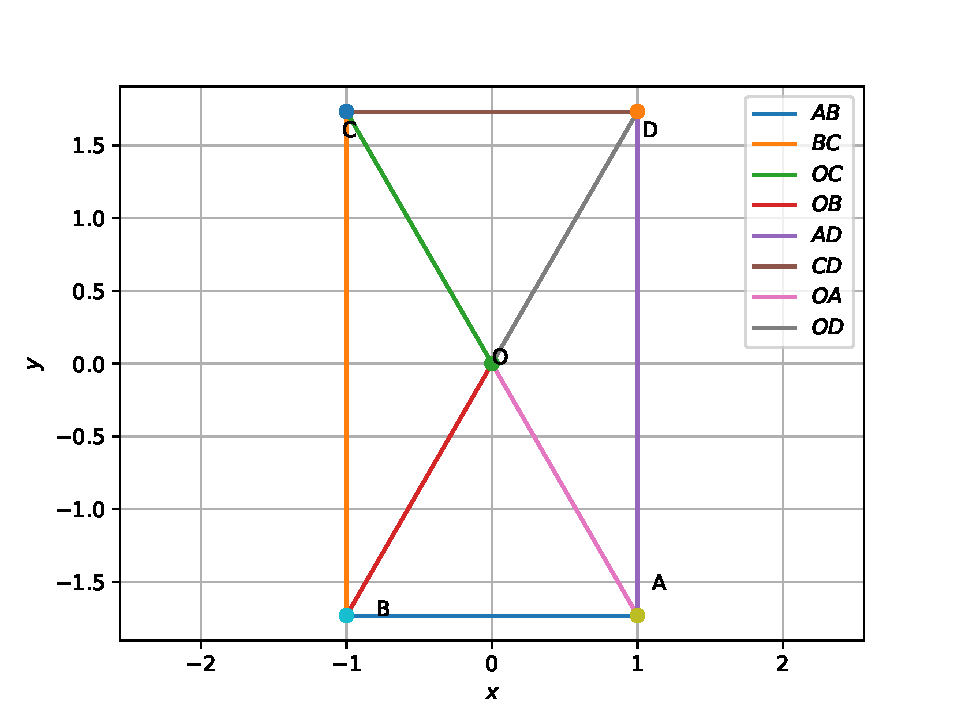
\includegraphics[width=1\columnwidth]{fig}
\caption{}
\end{figure}

\section{Construction}
\begin{tabular}{|c|c|c|}
  \hline
  \textbf{Point}&\textbf{Value}&\textbf{Description}\\
  \hline
  B&(2,0)&  Given point\\
  \hline
  A&(3,0)& Given point\\
  \hline
  
  
  
\end{tabular}









Given  equation is \begin{align}
y=x^2-5x+6=0
\end{align}




\begin{align}
x^2-5x-y+6=0
\end{align}
\begin{align}
\vec{x}^T\vec{Vx}+2\vec{U}^T\vec{x}+f=0
\end{align}
\begin{eqnarray}
V=\myvec{1&0\\ 0 &0} \; u=\myvec{\frac{-5}{2}\\\frac{-1}{2}} \;  f=6
\end{eqnarray}






Where  
\begin{eqnarray}
(\vec{V}\vec{q}+\vec{u})^T\vec{x}+\vec{u}^T\vec{q}+f=0
\end{eqnarray}
From the point 1
\begin{eqnarray}
\vec{Q_1}=\myvec{2\\0}
\end{eqnarray}

By substituting the point Q in the above equation
\begin{eqnarray}
	(\vec{V}\vec{q}+\vec{u})^T\vec{x}+\vec{u}^T\vec{q}+f=0
\end{eqnarray}




\begin{eqnarray}
(-1/2&-1/2)x\;+(-5/2&-1/2)\myvec{2\\0}+6=0
\end{eqnarray}
From above equation
\begin{eqnarray}
\vec{m_1}=\myvec{-1/2 & -1/2}
\end{eqnarray} 

From the point 2
\begin{align}
\vec{Q_2}=\myvec{3\\0}\
\end{align}
\begin{eqnarray}
(1/2 & -1/2)x\;+(-5/2&-1/2)\myvec{3\\0}+6=0
\end{eqnarray}
From above equation
\begin{eqnarray}
\vec{m_2}=\myvec{1/2&-1/2}
\end{eqnarray} 
\\
The angle between two vectors is given by 
\begin{eqnarray}
	\theta=cos^{-1}\frac{\vec{m_1}^T\vec{m_2}}{\norm{\vec{m_1}}\norm{\vec{m_2}}}
\end{eqnarray}

By substituting values of $\vec{m_1}$ and $\vec{m_2}$ in the following Equation 

\begin{eqnarray}
	cos^{-1}\theta=0
\end{eqnarray}


Angle between them is $\frac{\pi}{2}$




 
\end{document}
